\documentclass[10pt,a4paper]{article}
\usepackage[utf8]{inputenc}
\usepackage{amsmath}
\usepackage{amsfonts}
\usepackage{amssymb}
\usepackage{graphicx}
\usepackage{tikz}
\usepackage{parskip}
\usepackage[left=2cm,right=2cm,top=2cm,bottom=2cm]{geometry}
\usepackage{sectsty}

\sectionfont{\usefont{OT1}{phv}{b}{n} \sectionrule{0pt}{0pt}{-5pt}{3pt}}
\author{Songtuan Lin u6162630}
\title{Assignment 4}
\begin{document}
\maketitle

\section*{Question 1}
\subsection*{(a)}
According to the definition of conjugate function: $f^{*}(\mathbf{y}) = \displaystyle\sup_{\mathbf{x}}\{ \mathbf{x}^{T} \mathbf{y} - f(\mathbf{x}) \}$, for any $\mathbf{y}$ and $\mathbf{x} \in \mathcal{D}$, we have:
\begin{equation*}
	\begin{aligned}
		f^{*}(\mathbf{y}) &= \displaystyle\sup_{\mathbf{x}}\{ \mathbf{x}^{T} \mathbf{y} - f(\mathbf{x}) \} \\
		&\geq \mathbf{x}^{T} \mathbf{y} - f(\mathbf{x})
	\end{aligned} 
\end{equation*}
By moving the term $f(\mathbf{x})$ within above equation from right-hand side to left-hand side, we can verify that:
\begin{equation*}
	f^{*}(\mathbf{y}) + f(\mathbf{x}) \geq \mathbf{x}^{T} \mathbf{y}
\end{equation*}

\subsection*{(b)}
By substituting $\mathbf{y} = \mathbf{0}$ to $f^{*}(\mathbf{y})$, we have:
\begin{equation*}
	\begin{aligned}
		f^{*}(0) &= \displaystyle\sup_{\mathbf{x}} \{ -f(\mathbf{x}) \} \\
	\end{aligned}
\end{equation*}
We can multiple both side of above equation with $-1$, then, we get:
\begin{equation*}
	\begin{aligned}
		-f^{*}(0) &= - \displaystyle\sup_{\mathbf{x}} \{ -f(\mathbf{x}) \} \\
		&= \displaystyle\inf_{\mathbf{x}} \{ f(\mathbf{x}) \}
	\end{aligned}
\end{equation*}

\subsection*{(c)}
We can write the conjugate function of $f(\mathbf{x})$ as:
\begin{equation*}
	f^{*}(\mathbf{y}) = \displaystyle\sup_{\mathbf{x}} \{ \displaystyle\sum_{i = 1}^{n}(x_{i}y_{i} - \alpha_{i}\log{x_{i}}) \}
\end{equation*}
Suppose there exist a $\alpha_{i} \geq 0$, then, for any $y_{i}$, the term $x_{i} y_{i} - \alpha_{1} \log{x_{i}}$ can always reach infinity, \textit{i.e.} for any $y_{i}$, $(x_{i} y_{i} - \alpha_{1} \log{x_{i}}) \rightarrow \infty$ when $x_{i} \rightarrow 0$. Hence, we can always choose a $\mathbf{x}$ with $x_{i} \rightarrow 0$ and make $(x_{i} y_{i} - \alpha_{1} \log{x_{i}}) \rightarrow \infty$, which means, $f^{*}(\mathbf{y}) < \infty$ if $\alpha_{i} < 0$ for each $i$.

Now we can start to discuss the domain of $f^{*}$ under the situation $\alpha \prec 0$: Indeed, if there exist a $y_{i} > 0$, then, the term $x_{i} y_{i} - \alpha_{1} \log{x_{i}}$ will goes to infinity when $x_{i} \rightarrow \infty$. This is because $x_{i} y_{i} \rightarrow \infty$ along with $x_{i} \rightarrow \infty$ and $-\alpha_{i}\log{x_{i}}$ always greater than zero. Based on this observation, we can conclude the domain of $f^{*}$ is $\mathbf{y} \prec 0$.

Finally, we can start to find the conjugate function. We first notice that when $y_{i} < 0$ and $\alpha_{i} > 0$, the term $x_{i} y_{i} - \alpha_{1} \log{x_{i}}$ is a concave function over $x_{i}$. As a result, the function $g(\mathbf{x}) = \displaystyle\sum_{i = 1}^{n}(x_{i}y_{i} - \alpha_{i}\log{x_{i}})$ is also concave as it is a non-negative sum of concave functions, which means, $g(\mathbf{x})$ will reach the maximum at the point $\mathbf{x^{*}}$ that satisfied:
\begin{equation*}
	\nabla_{\mathbf{x}} g(\mathbf{x^{*}}) = 0
\end{equation*}
The above equation is equivalent to:
\begin{equation}
	y_{i} - \alpha_{i} \frac{1}{x_{i}} = 0 \quad i = 1, 2, \cdots, n
	\label{conjugate}
\end{equation}
Solving Equation \ref{conjugate}, we get:
\begin{equation*}
	x_{i} = \frac{\alpha_{i}}{y_{i}}
\end{equation*}
Therefore, the conjugate function is:
\begin{equation*}
	\begin{aligned}
		f^{*}(\mathbf{y}) &= \displaystyle\sup_{\mathbf{x}}(g(\mathbf{x})) \\
		&= \displaystyle\sum_{i = 1}^{n}(\alpha_{i} - \alpha_{i} \log{\frac{\alpha_{i}}{y_{i}}})
	\end{aligned}
\end{equation*}

\section*{Question 2}
\subsection*{(a)}
The original problem can be expressed as:
\begin{equation*}
	\displaystyle\min_{x} \quad \displaystyle\sum_{i = 1}^{n} |x - b_{i}|
\end{equation*}
with the objective function $f(x) = \displaystyle\sum_{i = 1}^{n} |x - b_{i}|$ and domain $x \in \mathcal{R}$. Indeed, we can reorder the terms within $f(x)$ as:
\begin{equation*}
	f(x) = |x - b^{*}_{1}| + |x - b^{*}_{2}| + \cdots + |x - b^{*}_{n}|
\end{equation*}
Where $b^{*}_{1}, b^{*}_{2} \cdots b^{*}_{n}$ is a reordered sequence generated from $b_{1}, b_{2} \cdots b_{n}$ and satisfied $b^{*}_{i} \leq b^{*}_{j}$ if $i < j$. By observing $f(x)$, we noticed that when $x$ satisfied $b^{*}_{i} \leq x < b^{*}_{i + 1}$, there is:
\begin{equation*}
	\begin{aligned}
		f(x) &= (x - b^{*}_{1}) + (x - b^{*}_{2}) + \cdots + (x - b^{*}_{i}) + (b^{*}_{i + 1} - x) + (b^{*}_{i + 2} - x) + \cdots + (b^{*}_{n} - x) \\
		&= (2i - n)x + (b^{*}_{i + 1} + b^{*}_{i + 2} + \cdots + b^{*}_{n}) - (b^{*}_{1} + b^{*}_{2} + \cdots +b^{*}_{i}) \\
		&= (2i - n)x + \sigma
	\end{aligned}
\end{equation*}
Where we have defined $\sigma = (b^{*}_{i + 1} + b^{*}_{i + 2} + \cdots + b^{*}_{n}) - (b^{*}_{1} + b^{*}_{2} + \cdots +b^{*}_{i})$. By observing $f(x)$, we first notice that when $i \leq \frac{n}{2}$, $f(x)$ is always a non-increasing function and when $i > \frac{n}{2}$, $f(x)$ is always non-decreasing. Additionally, $i$ is the index and hence, it must be an integer. Therefore, we can conclude that: 
\begin{enumerate}
	\item $f(x)$ is non-increasing when $i \leq \lfloor \frac{n}{2} \rfloor$.
	\item $f(x)$ is non-decreasing when $i \geq \lceil \frac{n}{2} \rceil$.
\end{enumerate}
Furthermore, since $i \leq \lfloor \frac{n}{2} \rfloor$ corresponding to the interval $x  < b^{*}_{\lfloor \frac{n}{2} \rfloor + 1} = b^{*}_{\lceil \frac{n}{2} \rceil}$ and $i \geq \lceil \frac{n}{2} \rceil$ corresponding to the interval $x \geq b^{*}_{\lceil \frac{n}{2} \rceil}$, we can conclude that $f(x)$ is non-increasing when $x < b^{*}_{\lceil \frac{n}{2} \rceil}$ and is non-decreasing when $x \geq b^{*}_{\lceil \frac{n}{2} \rceil}$. As a result, $f(x)$ reach the minimum at the optimal point $x = b^{*}_{\lceil \frac{n}{2} \rceil}$.

\subsection*{(b)}
We first notice that the function $\| x \mathbf{1} - \mathbf{b} \|_{2}$ have the same optimal point as $\| x \mathbf{1} - \mathbf{b} \|_{2}^{2}$, which means, they both reach the minimum at the same point $x$. Therefore, we can find this optimal point by solving the optimal problem:
\begin{equation*}
	\begin{aligned}
		\displaystyle\min_{x} & \quad \| x \mathbf{1} - \mathbf{b} \|_{2}^{2}
	\end{aligned}
\end{equation*}
Which is the same as:
\begin{equation*}
	\displaystyle\min_{x} \quad \displaystyle\sum_{i = 1}^{n} (x - b_{i})^{2}
\end{equation*}
It is easy to verify that the function $f(x) = \displaystyle\sum_{i = 1}^{n} (x - b_{i})^{2}$ is convex by checking $\nabla^{2}_{x} f(x) = 2n > 0$. Therefore, according to the first-order condition, $f(x)$ will reach the minimum at the optimal $x^{*}$ which satisfied:
\begin{equation*}
	\begin{aligned}
		\nabla_{x}f(x^{*}) &= \displaystyle\sum_{i = 1}^{n}2(x^{*} - b_{i}) \\
		&= 0
	\end{aligned}
\end{equation*}
The solution of this equation is:
\begin{equation*}
	x^{*} = \frac{1}{n} \displaystyle\sum_{i = 1}^{n} b_{i}
\end{equation*}
Hence, the optimal point for the original problem is also $x^{*} = \frac{1}{n} \displaystyle\sum_{i = 1}^{n} b_{i}$.

\subsection*{(c)}
By using the similar method as in (a), we can reorder the elements within $\mathbf{b}$ and reform the problem as:
\begin{equation*}
	\begin{aligned}
		\displaystyle\min_{x} & \quad \displaystyle\max_{i} \{ |x - b^{*}_{1}|, |x - b^{*}_{2}|, \cdots, |x - b^{*}_{n}| \}
	\end{aligned}
\end{equation*}
We first check the situation that $x \leq b^{*}_{1}$, we have:
\begin{equation*}
	\begin{aligned}
		\| x \mathbf{1} - \mathbf{b} \|_{\infty} &= \displaystyle\max \{ b^{*}_{1} - x, b^{*}_{2} - x, \cdots, b^{*}_{n} - x \} \\
		&= b^{*}_{n} - x \\
		&\geq b^{*}_{n} - b^{*}_{1}
	\end{aligned}
\end{equation*}
It can be seen that under this situation, $\| x \mathbf{1} - \mathbf{b} \|_{\infty}$ reach the minimum $b^{*}_{n} - b^{*}_{1}$ when $x = b^{*}_{1}$.  After that, we can check the situation that $b^{*}_{1} \leq x \leq b^{*}_{i}$, we have:
\begin{equation*}
	\begin{aligned}
		\| x \mathbf{1} - \mathbf{b} \|_{\infty} &= \displaystyle\max\{ x - b^{*}_{1}, x - b^{*}_{2}, \cdots, x - b^{*}_{i - 1}, b^{*}_{i} - x, b^{*}_{i + 1} - x, \cdots, b^{*}_{n} - x \} \\
		&= \displaystyle\max \{ x - b^{*}_{1}, b^{*}_{n} - x \}
	\end{aligned}
\end{equation*}
We first notice that the above equation hold for any $b^{*}_{i}$, hence, we can expand this equation to the condition that $b^{*}_{1} \leq x \leq b^{*}_{n}$:
\begin{equation*}
	\| x \mathbf{1} - \mathbf{b} \|_{\infty} = \displaystyle\max \{ x - b^{*}_{1}, b^{*}_{n} - x \}
\end{equation*}
Furthermore, we realize that when $x > \frac{b^{*}_{1} + b^{*}_{n}}{2}$, $x - b^{*}_{1} > b^{*}_{n} - x$ and when $x \leq \frac{b^{*}_{1} + b^{*}_{n}}{2}$, $x - b^{*}_{1} \leq b^{*}_{n} - x$. Therefore, we have:
\begin{equation*}
	\| x \mathbf{1} - \mathbf{b} \|_{\infty} = 
	\begin{cases}
		b^{*}_{n} - x & \quad x \leq \frac{b^{*}_{1} + b^{*}_{n}}{2} \\
		x - b^{*}_{1} & \quad x > \frac{b^{*}_{1} + b^{*}_{n}}{2}
	\end{cases}
\end{equation*}
Hence, $\| x \mathbf{1} - \mathbf{b} \|_{\infty}$ reach the minimum value $\frac{b^{*}_{n} - b^{*}_{1}}{2}$ at $x = \frac{b^{*}_{n} + b^{*}_{1}}{2}$. Finally, we can check the situation that $x \geq b^{*}_{n}$. Under this situation, $\| x \mathbf{1} - \mathbf{b} \|_{\infty}$ has the minimum $b^{*}_{n} - b^{*}_{1}$. Since $\frac{b^{*}_{n} - b^{*}_{1}}{2} < b^{*}_{n} - b^{*}_{1}$, we can then conclude that for any $x \in \mathcal{R}$, the optimal point for function $\| x \mathbf{1} - \mathbf{b} \|_{\infty}$ is: 
\begin{equation*}
	x = \frac{b^{*}_{n} + b^{*}_{1}}{2}
\end{equation*}
with the optimal value $\frac{b^{*}_{n} - b^{*}_{1}}{2}$.

\subsection*{(d)}
As the similar method been used in (b), we can first find the optimal point for the optimal problem:
\begin{equation*}
	\displaystyle\min_{x} \quad \| x \mathbf{a} - \mathbf{b} \|^{2}_{2}
\end{equation*}
Which is equivalent to the problem:
\begin{equation*}
	\displaystyle\min_{x} \quad \displaystyle\sum_{i} (a_{i}x - b_{i})^{2}
\end{equation*}
It is easy to verify that the function $f(x) = \displaystyle\sum_{i} (a_{i}x - b_{i})^{2}$ is convex as $\nabla_{x}^{2} f(x) = \displaystyle\sum_{i}2 a_{i}^{2} > 0$. Therefore, the optimal point $x^{*}$ must satisfied the first-order condition:
\begin{equation*}
	\begin{aligned}
		\nabla_{x} f(x^{*}) &= \displaystyle\sum_{i} 2a_{i}(a_{i}x - b_{i}) \\
		&= 0
	\end{aligned}
\end{equation*}
The solution of this equation is:
\begin{equation*}
	x^{*} = \frac{\displaystyle\sum_{i}a_{i} b_{i}}{\displaystyle\sum_{i} a_{i}^{2}}
\end{equation*}
Which means, the optimal point of the original problem is $x^{*} = \frac{\displaystyle\sum_{i}a_{i} b_{i}}{\displaystyle\sum_{i} a_{i}^{2}}$.

\section*{Q3}
\subsection*{(a)}
We can first the Lagrangian as:
\begin{equation*}
	\begin{aligned}
		\mathcal{L}(\mathbf{x}, \mathbf{r}) &= \displaystyle\sum_{i} \phi(r_{i}) - \nu^{T}(\mathbf{r} - \mathcal{A}\mathbf{x} + \mathbf{b}) \\
		&= \displaystyle\sum_{i} \phi(r_{i}) - \nu^{T} \mathbf{r} + \nu^{T} \mathcal{A} \mathbf{x} - \nu^{T} \mathbf{b}
	\end{aligned}
\end{equation*}
According to the Lagrangian, we can further write the Lagrange Dual Function as:
\begin{equation*}
	\begin{aligned}
		g(\nu) = \displaystyle\inf_{\mathbf{r}, \mathbf{x}} \{ \displaystyle\sum_{i} \phi(r_{i}) - \nu^{T} \mathbf{r} + \nu^{T} \mathcal{A} \mathbf{x} - \nu^{T} \mathbf{b} \}
	\end{aligned}
\end{equation*}
By inspecting the Lagrange Dual Function, we can find that if $\nu^{T} \mathcal{A} \neq 0$, $g(\nu)$ can easily approach to $-\infty$ as $\mathbf{x} \rightarrow \infty$ or $-\infty$. Therefore, the first condition that $\nu$ need to satisfied is:
\begin{equation}
	\nu^{t} \mathcal{A} = 0
\end{equation}
Therefore, the Lagrange Dual Function can be simplified as:
\begin{equation*}
	\begin{aligned}
		g(\nu) &= \displaystyle\inf_{\mathbf{r}} \{ \displaystyle\sum_{i} \phi(r_{i}) - \nu^{T} \mathbf{r} - \nu^{T} \mathbf{b} \} \\
		&= \displaystyle\inf_{\mathbf{r}} \{ \displaystyle\sum_{i} \phi(r_{i}) - \nu^{T} \mathbf{r} \} - \nu^{T} \mathbf{b} \\
		&= \displaystyle\inf_{\mathbf{r}} \{ \displaystyle\sum_{i} (\phi(r_{i}) - v_{i} r_{i}) \} - \nu^{T} \mathbf{b}
	\end{aligned}
\end{equation*}
As a result, the first thing we need to do to construct the Dual Problem is to solve $\displaystyle\inf_{\mathbf{r}} \{ \displaystyle\sum_{i} (\phi(r_{i}) - v_{i} r_{i}) \}$. In order to do so, we first notice that the element $r_{i}$ within $\mathbf{r}$ is independent with each other, therefore, we can first find the minimum of each single term: $\phi(r_{i}) - v_{i} r_{i}$ and then sum them together. Indeed, we can discuss the minimum of $\phi(r_{i}) - v_{i} r_{i}$ based on the following three cases:
\begin{enumerate}
	\item $r_{i} \leq -1$: Under this condition, the term $\phi(r_{i}) - v_{i} r_{i}$ become:
	\begin{equation*}
		\begin{aligned}
			\phi(r_{i}) - v_{i} r_{i} &= -r_{1} - 1 - \nu_{i} r_{i} \\
			&= (-\nu_{i} - 1) r_{i} - 1
		\end{aligned}
	\end{equation*}
	Based on this equation, it is easy to find out that of $\nu_{i} \geq -1$, $\phi(r_{i}) - v_{i} r_{i}$ reach the minimum $\nu_{i}$ at $r_{i} = -1$. By contrast, if $\nu_{i} < -1$, $\phi(r_{i}) - v_{i} r_{i} \rightarrow -\infty$ as $r_{i} \rightarrow -\infty$. Therefore, the second condition that $\nu$ must satisfied is: For each $\nu_{i}$:
	\begin{equation}
		\nu_{i} \geq -1
	\end{equation}
	\item $r_{i} \geq 1$: Under this condition, the term $\phi(r_{i}) - v_{i} r_{i}$ become:
	\begin{equation*}
		\phi(r_{i}) - v_{i} r_{i} = (1 - \nu_{i}) r_{i} - 1
	\end{equation*}
	By inspecting this equation, if $\nu_{i} \leq 1$, $\phi(r_{i}) - v_{i} r_{i}$ has the minimum $-\nu_{i}$ at the point $r_{i} = 1$. By contrast, if $\nu_{i} > 1$, $\phi(r_{i}) - v_{i} r_{i}$ goes to $-\infty$ along with $r_{i} -\rightarrow \infty$. As a result, the third condition that $\nu$ must satisfied is: For each $\nu_{i}$
	\begin{equation}
		\nu_{i} \leq 1
	\end{equation}
	\item $-1 \leq r_{i} \leq 1$: Under this condition, the term $\phi(r_{i}) - v_{i} r_{i}$ become:
	\begin{equation*}
		\phi(r_{i}) - v_{i} r_{i} = -\nu_{i} r_{i}
	\end{equation*}
	Indeed, under this condition, it is straightforward to figure out the minimum of $\phi(r_{i}) - v_{i} r_{i}$ is either $\nu_{i}$ or $-\nu_{i}$ according to the sign of $\nu_{i}$.
\end{enumerate}
As a result, we can find the minimum of $\phi(r_{i}) - v_{i} r_{i}$ over the entire range of $r_{i}$ by combining the above three conditions:
\begin{equation}
	\begin{aligned}
		\displaystyle\inf_{r_{i}}\{ \phi(r_{i}) - v_{i} r_{i} \} &= \displaystyle\min \{ -\nu_{i}, \nu_{i} \} \\
		&= - |\nu_{i}|
	\end{aligned}
	\label{inf}	
\end{equation}
With the constrain:
\begin{equation*}
	-1 \leq \nu_{i} \leq 1
\end{equation*}
Which is equivalent to:
\begin{equation}
	|\nu_{i}| \leq 1
	\label{c_1}
\end{equation}
and 
\begin{equation}
	\nu^{T} \mathcal{A} = 0
	\label{c_2}
\end{equation}
As a result, the Dual Function, accoeding to Equation \ref{inf}, \ref{c_1} and \ref{c_2},  can be written as:
\begin{equation}
	\begin{aligned}
		g(\nu) &= \displaystyle\sum_{i} -|\nu_{i}| - \nu^{T} \mathbf{b} \\
		&= - \| \nu \|_{1} - \nu^{T} \mathbf{b}
	\end{aligned}
\end{equation}
With the constrains: $|\nu_{i}| \leq 1$ for each $\nu_{i}$ and $\nu^{T} \mathcal{A} = 0$. Furthermore, since for each $\nu_{i}$ in $\nu$, there is $ |\nu_{1}| \leq 1$, we can rewrite this constrain as $\| \nu \|_{\infty} \leq 1$. As a result, the dual problem is:
\begin{equation*}
	\begin{aligned}
		\displaystyle\max_{\nu} \quad & - \| \nu \|_{1} - \nu^{T} \mathbf{b} \\
		\textsl{s.t.}  \quad & \| \nu \|_{\infty} \leq 1 \\
		& \nu^{T} \mathcal{A} = 0
	\end{aligned}
\end{equation*}

\subsection*{(b)}
As what we did in (a), we can first construct the Lagrangian:
\begin{equation*}
	\displaystyle\sum_{i} \phi(r_{i}) - \nu^{T} \mathbf{r} + \nu^{T} \mathcal{A} \mathbf{x} - \nu^{T} \mathbf{b}
\end{equation*}
and the Lagrange Dual Function:
\begin{equation*}
	g(\nu) = \displaystyle\inf_{\mathbf{r}} \{ \displaystyle\sum_{i} (\phi(r_{i}) - v_{i} r_{i}) \} - \nu^{T} \mathbf{b}
\end{equation*}
with constrain:
\begin{equation*}
	\nu^{T} \mathcal{A} = 0
\end{equation*}
Indeed, in order to find the minimum of $\displaystyle\sum_{i} (\phi(r_{i}) - v_{i} r_{i})$, we can also start with finding the minimum of each $\phi(r_{i}) - \nu_{i} r_{i}$ and then summing them together. As in (a), we also separate the discussion into following cases:
\begin{enumerate}
	\item $r_{i} \leq -1$: Under this condition, the term $\phi(r_{i}) - \nu_{i} r_{i}$ becomes:
	\begin{equation*}
		\phi(r_{i}) - \nu_{i} r_{i} = (-2 - \nu_{i}) r_{i} - 1
	\end{equation*}
	By inspecting this equation, we can find out that if $\nu_{i} \geq -2$, $\phi(r_{i}) - \nu_{i} r_{i}$ reach the minimum $\nu_{i} + 1$ at point $r_{i} = -1$. By contrast, if $\nu_{i} < -2$, $\phi(r_{i}) - \nu_{i} r_{i}$ will goes to $-\infty$ along with $r_{i} \rightarrow -\infty$. Therefore, for each $\nu_{i}$, it must satisfied:
	\begin{equation}
		\nu_{i} \geq -2
		\label{c_3}
	\end{equation}
	\item $r_{i} \geq 1$: Under this condition, the  term $\phi(r_{i}) - \nu_{i} r_{i}$ becomes:
	\begin{equation*}
		\phi(r_{i}) - \nu_{i} r_{i} = (2 - \nu_{i})r_{i} - 1
	\end{equation*}
	By inspecting this equation, we can find out that if $\nu_{i} \leq 2$, $\phi(r_{i}) - \nu_{i} r_{i}$ reach the minimum at point $r_{i} = 1$. By contrast, if $\nu_{i} > 2$, $\phi(r_{i}) - \nu_{i} r_{i}$ goes to $-\infty$ along with $r_{i} \rightarrow \infty$. Therefore, for each $\nu_{i}$, it also need to satisfied:
	\begin{equation}
		\nu_{i} \leq 2
		\label{c_4}
	\end{equation}
	\item $-1 \leq r_{i} \leq 1$: Under this condition, the term $\phi(r_{i}) - \nu_{i} r_{i}$ becomes:
	\begin{equation}
		\phi(r_{i}) - \nu_{i} r_{i} = r_{i}^{2} - \nu_{i} r_{i}
	\end{equation}
	We first notice that if we do not consider the range of $r_{i}$, $r_{i}^{2} - \nu_{i} r_{i}$ will reach the minimum $-\frac{\nu_{i}^{2}}{4}$ at the point $r_{i} = \frac{\nu_{i}}{2}$. Indeed, from constrain \ref{c_3} and \ref{c_4}, we have $-2 \leq \nu_{i} \leq 2$. Therefore, 
	\begin{equation*}
		-1 \leq \frac{\nu_{i}}{2} \leq 1
	\end{equation*}
	which located inside out assumption range of $r_{i}$. Hence, $\phi(r_{i}) - \nu_{i} r_{i}$ reach the minimum $-\frac{\nu_{i}^{2}}{4}$ at the point $r_{i} = \frac{\nu_{i}}{2}$.
\end{enumerate}
We can construct the minimum of $\phi(r_{i}) - \nu_{i} r_{i}$ over the entire range of $r_{i}$ by combining the above three cases:
\begin{equation*}
	\displaystyle\inf_{r_{i}}\{ \phi(r_{i}) - \nu_{i} r_{i} \} = \displaystyle\min \{ \nu_{i} + 1, 1 - \nu_{i}, -\frac{\nu_{i}^{2}}{4} \}
\end{equation*}
with the constrain $-2 \leq \nu_{i} \leq 2$ and $\nu^{T} \mathcal{A} = 0$. Indeed, we can plot the graph for these three terms as:
\begin{center}
	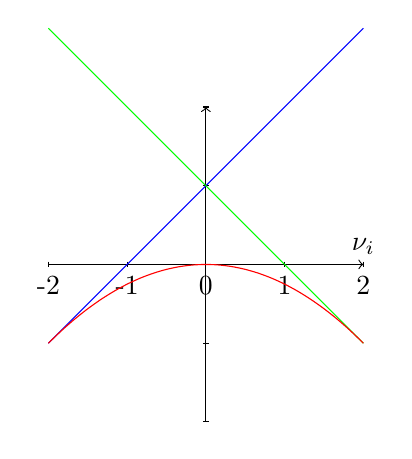
\begin{tikzpicture}
		\draw[->] (-2, 0) -- (2, 0) node[above] {$\nu_{i}$};
		\draw[->] (0, -2) -- (0, 2);
		\foreach \x in {-2,-1,0,1,2}
   			\draw[-] (\x cm,1pt) -- (\x cm,-1pt) node[anchor=north] {\x};
		\foreach \y in {-2,-1,0,1,2}
    			\draw (1pt,\y cm) -- (-1pt,\y cm) node[anchor=east] {};
		\draw[scale=1,domain=-2:2,smooth,variable=\x,blue] plot ({\x},{\x + 1});
		\draw[scale=1,domain=-2:2,smooth,variable=\x,green] plot ({\x},{1 - \x});
		\draw[scale=1,domain=-2:2,smooth,variable=\x,red] plot ({\x},{- \x*\x / 4});
	\end{tikzpicture}
\end{center}
It can be seen that within the interval $-2 \leq \nu_{i} \leq 2$, we have $\displaystyle\min \{ \nu_{i} + 1, 1 - \nu_{i}, -\frac{\nu_{i}^{2}}{4} \} = - \frac{\nu_{i}^{2}}{4}$. As a result, we have:
\begin{equation*}
	\displaystyle\inf_{r_{i}}\{ \phi(r_{i}) - \nu_{i} r_{i} \} = - \frac{\nu_{i}^{2}}{4}
\end{equation*}
Therefore, the Dual Function is:
\begin{equation*}
	\begin{aligned}
	g(\nu) &= \displaystyle\sum_{i} - \frac{\nu_{i}^{2}}{4} - \nu^{T} \mathbf{b} \\
	&= -\frac{1}{4} \| \nu \|_{2}^{2} - \nu^{T} \mathbf{b}
	\end{aligned}
\end{equation*}
Hence, the Dual Problem is:
\begin{equation*}
	\begin{aligned}
		\displaystyle\max_{\nu} \quad & -\frac{1}{4} \| \nu \|_{2}^{2} - \nu^{T} \mathbf{b} \\
		\textsl{s.t.} \quad & \| \nu \|_{\infty} \leq 2 \\
		& \nu^{T} \mathcal{A} = 0
	\end{aligned}
\end{equation*}

\section*{Q4}
\subsection*{(a)}
Since $\mathbf{p}(x)$ is the density of variable $x$, then, for $\mu_{1} \leq x \leq \mu_{2}$, we have:
\begin{equation*}
	\mathcal{P}(\mu_{1} \leq x \leq \mu_{2}) = \int_{\mu_{1}}^{\mu_{2}}\mathbf{p}(x)\mathrm{d}x
\end{equation*}
If we substitute variable $x$ with a new variable $t$ and satisfied: $x = at - b$, the above equation is equivalent to:
\begin{equation}
	\begin{aligned}
		\int_{\mu_{1}}^{\mu_{2}}p(x)\mathrm{d}x &= \int_{\frac{\mu_{1} + b}{a}}^{\frac{\mu_{2} + b}{a}}\mathbf{p}(at - b)\mathrm{d}(at-b) \\
		&= \int_{\frac{\mu_{1} + b}{a}}^{\frac{\mu_{2} + b}{a}} a \mathbf{p}(at - b) \mathrm{d}t
	\end{aligned}
	\label{4a_1}
\end{equation}
Recalling that $y = \frac{x + b}{a}$, therefore, the following equation always holds:
\begin{equation}
	\mathcal{P}(\mu_{1} \leq x \leq \mu_{2}) = \mathcal{P}(\frac{\mu_{1} + b}{a} \leq y \leq \frac{\mu_{2}+ b}{a})
	\label{4a_2}
\end{equation}
Combining Equation \ref{4a_1} and \ref{4a_2}, we have:
\begin{equation*}
	\begin{aligned}
		\mathcal{P}(\frac{\mu_{1} + b}{a} \leq y \leq \frac{\mu_{2}+ b}{a}) &= \mathcal{P}(\mu_{1} \leq x \leq \mu_{2}) \\
		&= \int_{\mu_{1}}^{\mu_{2}}\mathbf{p}(x)\mathrm{d}x \\
		&= \int_{\frac{\mu_{1} + b}{a}}^{\frac{\mu_{2} + b}{a}} a \mathbf{p}(at - b) \mathrm{d}t
	\end{aligned}
\end{equation*}
This equation indicated that the density of $y$ is $\mathbf{p}_{y} = a \mathbf{p}(ay - b)$. Therefore, we can write down the log-likelihood for $\{ y_{1}, y_{2}, \cdots, y_{n} \}$ as:
\begin{equation*}
	\begin{aligned}
		\mathcal{L} &= \log \displaystyle\prod_{i = 2}^{n}{\mathbf{p}_{y_{i}}} \\
		&= \log \displaystyle\prod_{i = 1}^{n}{a \mathbf{p}(ay_{i} - b)} \\
		&= \displaystyle\sum_{i = 1}^{n}\log{a \mathbf{p}(ay_{i} - b)} \\
		&= n \log{a} + \displaystyle\sum_{i = 1}^{n} \log{\mathbf{p}(a y_{i} - b)}
	\end{aligned}
\end{equation*}
As a result, the maximize-likelihood optimized problem can be expressed as:
\begin{equation}
	\begin{aligned}
		\displaystyle\max_{a, b} \quad & n \log{a} + \displaystyle\sum_{i = 1}^{n} \log{\mathbf{p}(a y_{i} - b)} \\
		\textsl{s.t.} \quad & a > 0
	\end{aligned}
	\label{5_a}
\end{equation}
Since $\mathbf{p}$ is log-concave and $ay_{i} - b$ is linear function, the term $\displaystyle\sum_{i = 1}^{n} \log{\mathbf{p}(a y_{i} - b)}$ is concave. Furthermore, as $n \log{a}$ is also concave, the whole objective function $n \log{a} + \displaystyle\sum_{i = 1}^{n} \log{\mathbf{p}(a y_{i} - b)}$ is concave. Additionally, the constrain $a > 0$ define a convex set, hence, this optimized problem is a convex optimize problem.

\subsection*{(b)}
By substituting $\mathbf{p}(x) = e^{-2 |x|}$ to Problem \ref{5_a}, we have:
\begin{equation*}
	\begin{aligned}
		n \log{a} + \displaystyle\sum_{i = 1}^{n} \log{\mathbf{p}(a y_{i} - b)} &= n \log{a} + \displaystyle\sum_{i = 1}^{n} \log{e^{-2|ay_{i} - b|}} \\
		&= n \log{a} - 2 \displaystyle\sum_{i = 1}^{n}|ay_{i} - b|
	\end{aligned}
\end{equation*}
Hence, the original problem becomes:
\begin{equation*}
	\begin{aligned}
		\displaystyle\min_{a, b} \quad & 2 \displaystyle\sum_{i = 1}^{n}|ay_{i} - b| - n \log{a} \\
		\textsl{s.t.} \quad & a > 0
	\end{aligned}
\end{equation*}
Since the objective function is convex, we can first fix $a$ and minimize the objective function over $b$. Therefore, we can solve the original problem by first solving the following optimal problem:
\begin{equation*}
	\begin{aligned}
		\displaystyle\min_{b} \quad & 2 \displaystyle\sum_{i = 1}^{n}|ay_{i} - b| - n \log{a} \\
	\end{aligned}
\end{equation*}
Which is equivalent to the problem:
\begin{equation*}
	\begin{aligned}
		\displaystyle\min_{b} \quad & \displaystyle\sum_{i = 1}^{n}|ay_{i} - b| \\
	\end{aligned}
\end{equation*}
Furthermore, since $|ay_{i} - b| = |b - ay_{i}|$, we can further reformat the problem as:
\begin{equation*}
	\displaystyle\min_{b} \quad \| b \mathbf{1} - a \mathbf{y} \|
\end{equation*}
where $\mathbf{y} = \begin{bmatrix}
y_{1} & y_{2} & \cdots & y_{n}
\end{bmatrix}^{T}$. This optimize problem is  the same as Question 2(a). Therefore, we can directly use the result of Question 2(a): The optimal point is
\begin{equation*}
	b^{*} = a y^{*}_{\lceil \frac{n}{2} \rceil}
\end{equation*}
Where $y^{*}_{1}, y^{*}_{2}, \cdots, y^{*}_{n}$ is a reorder sequence of $y_{1}, y_{2}, \cdots, y_{n}$ which satisfied, for any $i < j$:
\begin{equation*}
	y^{*}_{i} \leq y^{*}_{j}
\end{equation*}
After we have find out the optimal value of $b$, we can solve the original problem by solving:
\begin{equation*}
	\begin{aligned}
		\displaystyle\min_{a} \quad & 2 \displaystyle\sum_{i = 1}^{n}|a(y_{i} - y^{*}_{\lceil \frac{n}{2} \rceil})| - n \log{a} \\
		\textsl{s.t.} \quad & a > 0
	\end{aligned}
\end{equation*}
Since $a > 0$ is equivalent to the domain of $\log{a}$, the problem is equivalent to:
\begin{equation*}
	\displaystyle\min_{a} \quad 2a \displaystyle\sum_{i = 1}^{n}|y_{i} - y^{*}_{\lceil \frac{n}{2} \rceil}| - n \log{a}
\end{equation*}
We can denote $c = \displaystyle\sum_{i = 1}^{n}|y_{i} - y^{*}_{\lceil \frac{n}{2} \rceil}|$. It is obvious that $c \geq 0$, therefore, the function $f_{0}(a) = 2ca - n \log{a}$ is convex as $\nabla_{a}^{2} f_{0}(a) \geq 0$. As a result, the optimal point $a^{*}$ should satisfied the first-order condition that:
\begin{equation*}
	\nabla_{a}f_{0}(a*) = 0
\end{equation*}
The solution of this equation is:
\begin{equation*}
	\begin{aligned}
		a^{*} &= \frac{n}{2c} \\
		&= \frac{n}{2 \displaystyle\sum_{i = 1}^{n}|y_{i} - y^{*}_{\lceil \frac{n}{2} \rceil}|}
	\end{aligned}
\end{equation*}
Hence, in conclusion, the optimal point is:
\begin{equation*}
	\begin{cases}
		a^{*} = \frac{n}{2 \displaystyle\sum_{i = 1}^{n}|y_{i} - y^{*}_{\lceil \frac{n}{2} \rceil}|} \\
		b^{*} = a^{*} y^{*}_{\lceil \frac{n}{2} \rceil}
	\end{cases}
\end{equation*}
\end{document}